% Source : http://texblog.net/latex-archive/maths/logic-tikz/

\documentclass{article}
	\usepackage{tikz}
	\usetikzlibrary{matrix}


\begin{document}

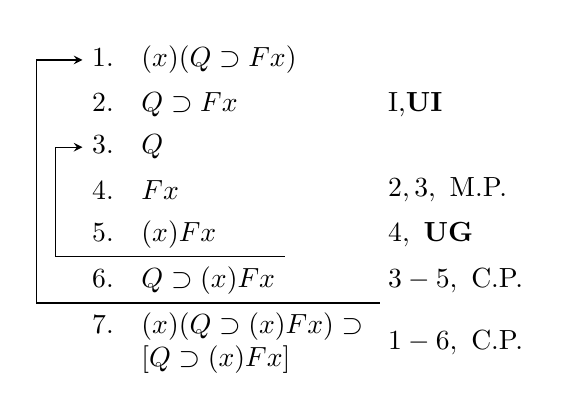
\begin{tikzpicture}[every node/.style={anchor=west}]
	\matrix (m) [
		matrix of math nodes,
		nodes in empty cells
	]{
		\quad & 1.\quad (x)(Q\supset Fx) & \\
		      & 2.\quad Q\supset Fx      & \textrm{I,\textbf{UI}} & \\
		      & 3.\quad Q \\
		      & 4.\quad Fx               & 2, 3, \textrm{ M.P.}\\
		      & 5.\quad (x)Fx            & 4, \textrm{ \textbf{UG}} \\
		      & 6.\quad Q\supset(x)Fx    & 3-5, \textrm{ C.P.} \\
		      & 7.\quad \parbox[t]{2.9cm}{%
					$(x)(Q\supset(x)Fx)\supset$\\
					$[Q\supset(x)Fx]$ %
				}                        & 1-6, \textrm{ C.P.}\\
	};
	\draw[-stealth] (m-7-2.north east)
		-| (m-1-1.west) |- (m-1-2);
	\draw[-stealth] (m-6-2.north east)
		-| (m-3-1.east) |- (m-3-2);
\end{tikzpicture}

\end{document}
